\chapter{Data collection}
\label{chap:methods}

\section{Introduction}

The analyses in chapters %\chapref{}, \chapref{}… 
use morphological and ecological data sets which I compiled for xx specimens representing xx species of small mammals. This chapter describes how the data were collected and checked for errors. First I outline how I compiled my morphological data set from museum specimens and secondly I describe the sources which contributed to my ecological dataset. Subsequent chapters will refer to both of these data sources but I will only describe the methods I used for their creation in detail here. Other methods I used which have specific relevance to subsequent chapters are described in those chapters.   

\section{Study species}
I collected morphological measurements of xxx species from  four mammalian orders; Afrosoricida, Erinaceomorpha, Soricomorpha and Notoryctemorphia comprising seven families of mammals; tenrecs (Tenrecidae), golden moles (Chrysochloridae), hedgehogs and gymnures(Erinaceidae), shrews (Soricidae), solenodons (Solenodontidae), moles and desmans(Talpidae) and marsupial moles (Notoryctidae).
My aim was to include measurements of all tenrecs and their sister taxa, golden moles.  For my  comparative species from other mammalian orders, I chose a random sample of xx taxa which have been previously identified as convergent with tenrecs \citep[e.g.][]{Gould1966, Symonds2005, Poux2008, Olson2013}. I followed the taxonomy in Wilson and Reeder's Mammal Species of the World (MSW) \citeyearpar{Wilson2005}. I used phylogenies for each order to select, at random, species representing the main sub-branches of each order which also represented the morphological diversity of that order. For example, within the Soricomorpha, I included both species of \textit{Solenodon} but only xx (out of a total of xx) species of \textit{Crocidura} as the former genus represents a separate subgroup to the rest of the order. 
%*****************************************
%Come back and rephrase this setion
%*****************************************

\section{Taxonomy}

Although MSW is a comprehensive mammalian taxonomic reference, it does not include some known species. For example, Wilson and Reader \citeyearpar{Wilson2005} record 30 species of tenrec but more recent studies indicate that there are now 34 recognised species of tenrec \citep{Olson2013}. The additional species belong to the shrew tenrec (\textit{Microgale}) genus and represent either recognition of cryptic species boundaries \citep{Olson2004} or discovery of new species \citep{Goodman2006, Olson2009}. Only one of these four recent additions to the \textit{Microgale} genus, \textit{M. jobihely}, was present in museum collections and therefore I could not include the three other newly recognised species in my analyses.

As MSW does not include all known species, I used the International Union for the Conservation of Nature \citep{IUCN2012} as an additional reference for the taxonomy and species diversity of each group. Table \ref{tab:species.measured} outlines the number of species I measured from each family and how this sample relates to the overall number of species in that group as recorded by both MSW and the IUCN.

%Species.measured table

\begin{table}[h]
\caption[Summary of species measured] %this appears in the table of contents
{The number of species I measured in each family compared to the total number of species in that family according to two sources; \citep{Wilson2005} and \citep{IUCN2012}}
\begin{tabular}{llccc}
\textbf{Order} & \textbf{Family} & \textbf{Species measured} & \textbf{Species in MSW} & \textbf{Species in IUCN} \\
%----------------------------------------------------
Afrosoricida & Tenrecidae & X & 30 & 34\\
%-------------------------------------------------
Afrosoricida & Chrysochloridae & X & 21 & 21\\
%----------------------------------------------------
Erinaceomorpha & Erinaceidae & X & 24 & X\\
%----------------------------------------------------
Soricomorpha & Soricidae & X & 376 & X\\
%----------------------------------------------------
Soricomorpha & Solenodontidae & X & 4 & X\\
%----------------------------------------------------
Soricomorpha & Talpidae & X & 39 & X\\
%----------------------------------------------------
Notoryctemorphia & Notoryctidae & X & 2 & X\\
%-----------------------------------------------
\end{tabular}
\label{tab:species.measured}
\end{table}

%----------------------------------------------------------------
\section{Morphological data set}
To construct my morphological data set, I used museum specimens of my study species housed at five different institutions. I compiled morphological data using two complementary approaches; linear measurements using calipers and 2D landmark-based geometric morphometrics.

\subsection{\normalfont{Museums visited}}

I measured and photographed the skulls, limbs and skins of tenrecs and the species they convergently resemble using the collections of five different museums; the Natural History Museum London (NHML), the Smithsonian Institute Natural History Museum (SI), the American Museum of Natural History (AMNH), Harvard’s Museum of Comparative Zoology (MCZ) and the Field Museum of Natural History (FMNH), Chicago. Between January and September 2013, I spent 9 weeks working in these collections and collected data from xxx skulls, xxx limbs and xxx skins of xxx species. 

\subsection{\normalfont{Museums label data}}
I recorded all the data on the specimen labels including any handwritten or printed notes which had been added by other users of the collection. The label data included the museum specimen ID number, genus, species, sex, collector’s name, the date and location of where the specimen was collected. Some of the labels attached to skins had additional information such as the body, tail, hind foot and ear lengths as well as the body mass of the live individual. 
The level of detail recorded on the labels varied considerably (figure \ref{fig:museum.labels}). For example recently collected specimens were more likely to have detailed information about the collection location, and some specimens did not have even basic information such as the sex recorded. 

%Museum label pictures

\begin{figure} 
  \centering
  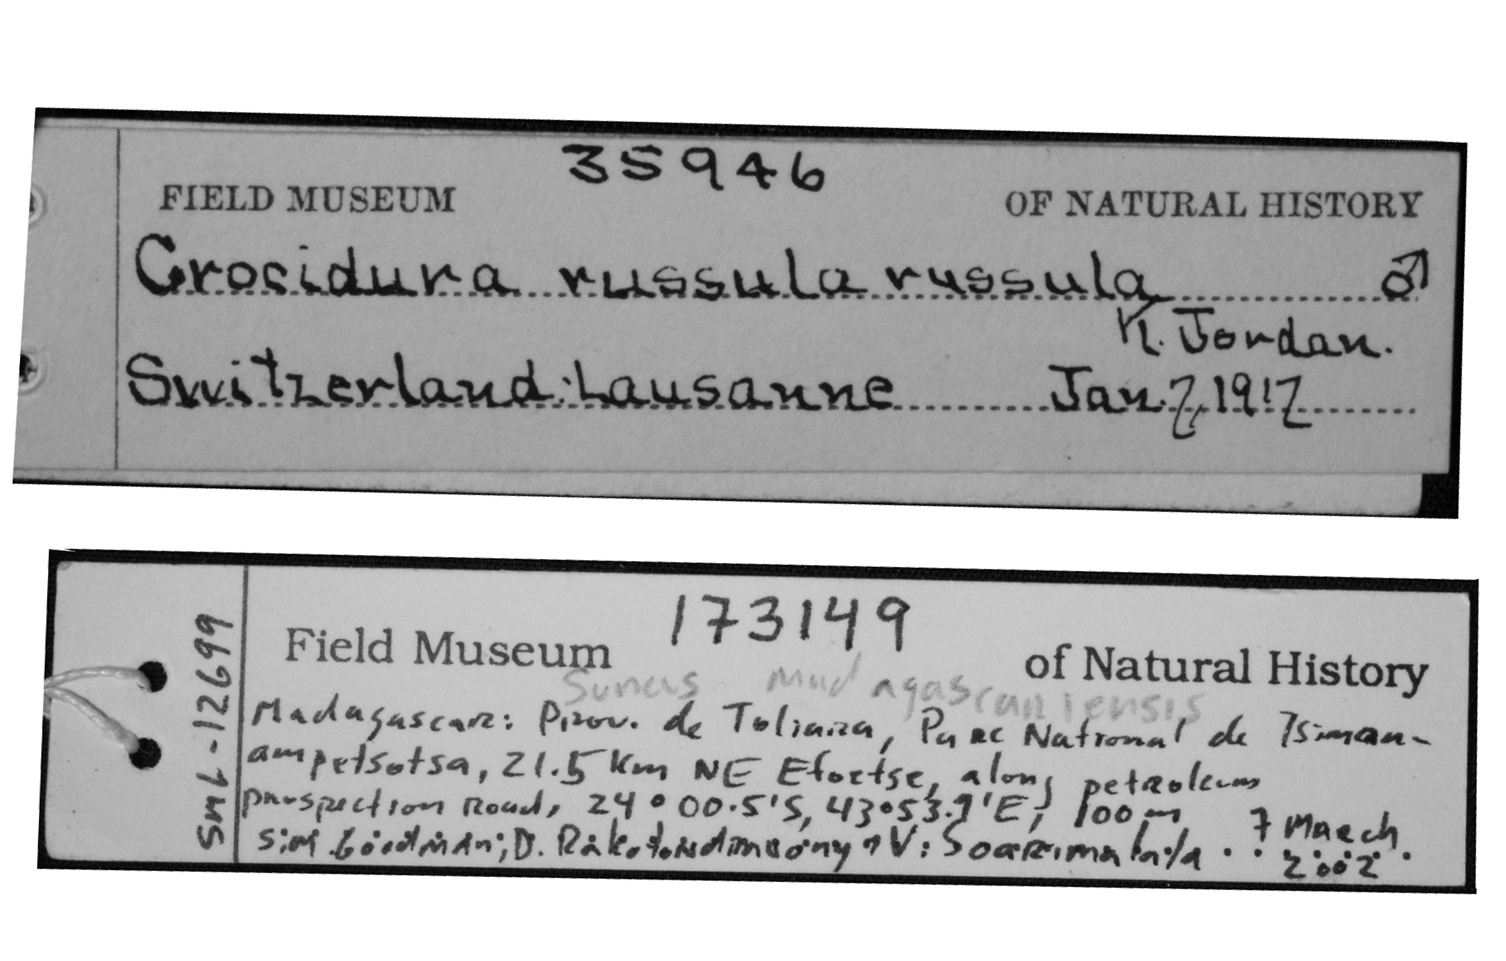
\includegraphics[width = 30cm, height = 10cm, keepaspectratio=true]{Methods/figures/labels.png}
    \caption[Examples of museum labels]%this is what appears in table of contents
    {Examples of the variation in the detail of information which is available from museum labels}%this is under the figure
  \label{fig:museum.labels}
  \end{figure}
  
%------------------------------------------------
\section{Linear measurements}

Using a 15mm digital calipers (Mitutoyo Absolute digimatic calipers), I took 20 measurements of the skulls and mandibles (table \ref{tab:sk.measurements}) and 19 measurements of the limbs (table \ref{limb.measurements}). My choice of which measurements to include was based on three main criteria; 1) their relevance to biological and ecological traits such as diet specialisation and locomotory adaptation, 2) their usefulness for assessing the overall shape and size of the specimen and 3) the ease with which they could be repeated both within and among specimens from different species. 
Figures x-x depict the linear measurements of skulls and figures xx show the limb measurements.

%******************************
%I need to put in diagrams here
%I need to fill in these tables
%******************************************
% Skull and mandible measurements
\begin{table}[h]
\caption[Description of the skull and mandible measurements]
		{Skull and mandible measurements}% add to this caption
\begin{tabular}{lll}
\textbf{Abbreviation} & \textbf{Measurement} & \textbf{Description}\\
\end{tabular}
\label{tab:sk.measurements}
\end{table}

%-----------------------------------------
% Limb measurements
\begin{table}[h]
\caption[Description of the limb measurements]
		{Limb measurements} % add to this caption
\begin{tabular}{lll}
\textbf{Abbreviation} & \textbf{Measurement} & \textbf{Description}\\
\end{tabular}
\label{tab:limb.measurements}
\end{table}

%*****************************
%Figures of the measurements
%****************************

I took each linear measurement three times, cycling through all 20 skull or 19 limb measurements then repeating the cycle to avoid measuring the same variable twice in a row. Small measurements (<2 mm) are particularly prone to high error rates \citep{Cardini2008}. Therefore, I took five separate replicates of some of the variables which were most prone to errors (marked with PUT IN SYMBOL in tables \ref{tab:sk.measurements} and \ref{tab:limb.measurements}). These included four of the skull measurements (PWa, IncisorH, IFD and IFcanal) and five of the limb measurements (FemD, TibD, HumD, UlnD, RadD). 
Five replicates should give a more reliable median value because even if there are one or two outlying measurements there should be at least three replicates which are in close agreement.
%-----------------------------------------------

\section{Landmark morphometrics}
\subsection{\normalfont{Photographic setup}}
In order to get 2D landmarks for my specimens, I first had to photograph them. I used photographic copy stands consisting of a camera attachment with an adjustable height bar, a flat stage on which to place the specimen and an adjustable light source to either side of the stage. I used the copy stands that were available at each museum which differed in how the camera height was adjusted and in the light sources available.
To take the light variability into account, on each day I took a picture of a white sheet of paper and used the custom white balance function on the camera to set the image as the baseline “white” measurement for those particular light conditions.

\subsection{\normalfont{Photographing specimens}}
I photographed the specimens with a Canon EOS 650D camera fitted with either an EF 100mm f/2.8 Macro USM lens (skulls and limbs) or EFS 18-55mm lens (skins). I used a remote control (h\"ahnel Combi TF) to take the photos to avoid shaking the camera and distorting the images. I photographed the specimens on a black material background. I placed the light source from the top left-hand corner of the picture and positioned a piece of white card on the bottom right side of the specimen which reflected the light back onto the specimen and minimised any shadows (figure \ref{fig:camera} below).

%----------------------------------------------
%Camera picture
\begin{figure}[h] 
  \centering
  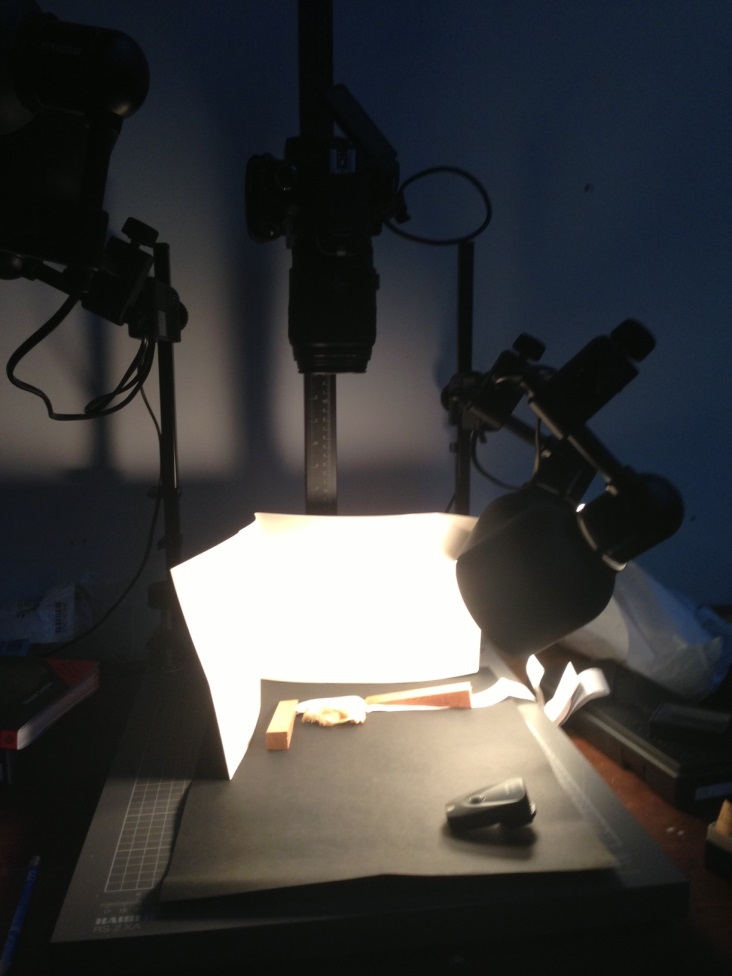
\includegraphics[keepaspectratio=true]{Methods/figures/camera_setup.jpg}
    \caption[Photographic set up]%this is what appears in table of contents
    {Photographic set up for taking images of my skulls. The camera (above centre) is fitted to a copy stand, the light source is directed from the top-left corner of the image and the white card reflects the light back onto the skull. }%this is under the figure
  \label{fig:camera}
  \end{figure}
%-------------------------------------------------
I made small bean bags (12 x 5cm) from the same black material as the background and filled them with plastic beads. I used these bags as necessary to hold the specimens in position while being photographed. For example, when taking pictures of the lateral view of skulls, I placed one bean bag under the nose of the skull and another bag lying along the top (cranial) side of the skull to ensure that the side I was photographing lay in a flat plane relative to the camera and did not tilt in any direction. 
I used the grid-line function on the live-view display screen of the camera to position the specimens in the centre of each image. 

\subsection{\normalfont{Skulls}}
I photographed the skulls in three views; dorsal (top of the cranium), ventral (underside of the skull with the palate roof facing uppermost) and lateral (right side of the skull). I also photographed the outer (buccal) side of the right mandible. When the right side of either the skull or mandibles were damaged or incomplete, I photographed the left sides and later reflected the images so that they could be compared to pictures of the right sides \citep[e.g.][]{Barrow2008}.

%Probably need a disclaimer somewhere about not being interested/ worried about bilateral asymmetry and also a quick test.

\subsection{\normalfont{Limbs}}
Initially, I tried to take pictures of the limbs in similar orientations to the skulls (dorsal, ventral and lateral). However, there was considerable variation in how the limbs were preserved. For example, some limbs were still articulated while others had fragmented bones. It therefore proved impossible to place the limb bones in consistent orientations that would be comparable across species. Similarly, the small size of some limbs, combined with the frequently incomplete nature of postcranial museum collections, made landmark-based morphometric analyses of any limb pictures impractical. Therefore, I photographed the fore- and hind-limb bones in outer (the side facing away from the rest of the body) and inner (the side facing in towards the centre of the body) views for reference purposes only.

\subsection{\normalfont{Skins}}
As I was limited by the maximum camera height available on the copy stands, most skins were too large to be photographed with the 100mm macro lens. Therefore, I used an EFS 18-55mm lens to take pictures of the skins. I photographed skins in the same three orientations as the skulls; dorsal (the upper surface of the animal), ventral (the belly side of the skin) and lateral (right flank of the animal with the skin held in position using bean bags). The dorsal and ventral views give very approximate estimates of the overall body shape of the animal. The lateral views are less biologically relevant since the taxidermic process is unlikely to produce specimens which represent the true body height of the animal.

\subsection{\normalfont{Saving and processing images}}
Photographs were captured and saved in a raw file format. Before using the pictures for morphometric analyses, I converted the raw files to binary (grey scale) images and re-saved them as TIFF files. The black and white pictures were more useful for later analyses since I was not interested in including any colour comparisons and it is easier to see some biological features in binary images. TIFF files were the most appropriate to use for my morphometric analyses as they are uncompressed (in comparison to JPEG) images and therefore there is less chance of any picture distortions which may affect later analyses \citep{HERC2013}.

\subsection{\normalfont{Landmark placement on images}}
%I need a general “this is morphometrics” overview at some stage; it might fit in here?

I conducted geometric morphometric analyses of my skull and mandible photographs. I used a combination of landmark and semilandmark analysis approaches to assess the shape variability of the specimens. In contrast to detailed morphometric studies of single taxa (e.g. Refs), the interspecific and comparative nature of my work limited the number of points which could be reliably identified as landmarks in all species….
%*******************************
%Tidy up this section
%********************************
I used the TPS software suite \citep{Rohlf2013} to digitise landmarks and curves on my pictures. I set the scale on each pictures individually to standardise for the different camera heights I used when photographing my specimens. I created separate data files for each of my morphometric analyses (three views of skulls and lateral view of mandibles). I digitised landmarks and semilandmark points on each picture individually.

When combining landmark and semi-landmark approaches, there is a potential problem of over-sampling the curves (REFS). To determine the number of semilandmark points required to adequately summarise the curves in my data sets,  I followed the method outlined by MacLeod \citeyearpar{MacLeod2012}. For each data set I chose a random selection of pictures of specimens which represented the breadth of the morphological data (i.e. specimens from each sub-group of species).  I drew the appropriate curves on the each specimen and over-sampled the number of points on the curves. I measured the length of the line and regarded that as the 100\%, true length of that outline. I then re-sampled the curves with decreasing numbers of points and measured the length of the outlines. I calculated the length of each re-sampled curve as a percentage of the total length of the curve and then found the average percentage length for across all of the specimens in my test file. I continued this process until I found the minimum number of points that gave a curve length which was at least 96\% accurate.  I repeated these curve-sampling tests for each analysis to determine the minimum number of semilandmark points which would give accurate representations of morphological shape.
After creating my files with the landmarks and semilandmarks placed on each picture, I built sliders files \citep{Zelditch2012} to specify which points should be treated as semilandmarks in further analyses. After landmarking and building sliders files, I used R v3.02 \citep[R Development Core]{Team2013} for all subsequent statistical analyses.



